% =====================================================================
% Mirante dos Dados — Working Paper #8
% O Benefício Emergencial de Manutenção do Emprego e da Renda (BEm)
% e a Resiliência do Mercado Formal Brasileiro Durante a Pandemia
% de COVID-19: Evidência de Microdados RAIS (2017–2022)
%
% Autor: Leonardo Chalhoub
% Versão: 0.1 — SKELETON 2026-04-28 (pós-Conselho)
%
% Status:
%   [✓] Bronze RAIS íntegra (2.06 B linhas, 40 anos, fix per-year reader)
%   [✓] Silver temática silver_rais_bem_panel (município × CNAE × ano)
%   [✓] 3 money shots geradas (VIZ-1, VIZ-2, VIZ-3)
%   [✓] 5 ADRs documentando schema drift e limitações
%   [✓] Sensibilidade SP 1986 notebook diagnostics
%   [ ] Modelos DiD/TWFE rodados — silver populada → próximo passo
%   [ ] Robustness checks (placebo, sensitivity, falsification) — TODO
%   [ ] Revisão sistemática literatura BEm — TODO (alerta Conselho Finanças)
%
% Compilação: pdflatex articles/rais-bem-covid.tex (2x)
% =====================================================================

\documentclass[12pt,a4paper,oneside]{article}

\usepackage[T1]{fontenc}
\usepackage[utf8]{inputenc}
\usepackage[brazilian]{babel}
\usepackage{newtxtext}
\usepackage{newtxmath}
\usepackage[section]{placeins}
\usepackage[a4paper,top=3cm,bottom=2cm,left=3cm,right=2cm]{geometry}
\usepackage{setspace}
\usepackage{indentfirst}
\usepackage{titlesec}
\usepackage{caption}
\usepackage{booktabs}
\usepackage{array}
\usepackage{multirow}
\usepackage{graphicx}
\usepackage[colorlinks=true,
            urlcolor=blue!60!black,
            linkcolor=black,
            citecolor=black,
            breaklinks=true]{hyperref}
\usepackage{url}
\usepackage{xurl}
\usepackage{float}
\usepackage{tcolorbox}
\usepackage{amsmath}

\graphicspath{{rais-figures/}}

\onehalfspacing
\setlength{\parindent}{1.25cm}
\setlength{\parskip}{0pt}

\titleformat{\section}{\normalfont\bfseries\large\uppercase}{\thesection}{0.6em}{}
\titleformat{\subsection}{\normalfont\bfseries\normalsize}{\thesubsection}{0.6em}{}

\title{
  \vspace{-1.5cm}
  {\large \textbf{Mirante dos Dados --- Working Paper \#8}}\\[0.3cm]
  \textbf{O Benefício Emergencial de Manutenção do Emprego e da Renda (BEm)}\\
  \textbf{e a Resiliência do Mercado Formal Brasileiro Durante a Pandemia de COVID-19}\\
  {\normalsize Evidência de Microdados RAIS (2017--2022)}
}
\author{Leonardo Chalhoub\thanks{MSc em Engenharia de Dados (UFRJ COPPE), 2023.
Pesquisador independente, Mirante dos Dados.
Replicação completa em \url{https://github.com/leonardochalhoub/mirante-dos-dados-br}.
\textit{Versão 0.1 --- skeleton} construído após auditoria de 40 anos de microdados
RAIS íntegros (commit \texttt{a334238} a \texttt{2158d65}, ADRs 001--005),
deliberação do Conselho do Mirante (2026-04-28), e validação de silver temática
\texttt{mirante\_prd.silver.rais\_bem\_panel}. Agradecimentos ao Conselho do
Mirante (Eng. Software, Finanças, Administração, Design).}}
\date{Versão 0.1 --- 28 de abril de 2026 (skeleton)}

\begin{document}
\maketitle

% =====================================================================
\begin{abstract}
\noindent
A pandemia de COVID-19 representou o maior choque adverso ao mercado de
trabalho global desde a Grande Depressão. No Brasil, o governo respondeu com
a Medida Provisória 936/2020, posteriormente convertida na Lei 14.020/2020,
criando o Benefício Emergencial de Manutenção do Emprego e da Renda (BEm).
O programa permitiu suspensão temporária de contratos e redução proporcional
de jornada/salário com subsídio público, cobrindo aproximadamente 10 milhões
de trabalhadores formais.

Este trabalho avalia o efeito causal do BEm sobre a preservação de vínculos
empregatícios formais entre 2020 e 2022, usando microdados RAIS Vínculos
Públicos completos (1985--2024, 2,06 bilhões de vínculos-ano). A estratégia
identificacional explora a heterogeneidade de exposição setorial
(\textit{difference-in-differences} com tratamento intensivo) entre setores
elegíveis ao BEm e setores essenciais não-elegíveis.

Os resultados preliminares indicam que o emprego formal brasileiro foi
notavelmente resiliente em 2020: a queda de vínculos ativos em 31/12 foi de
apenas $-1{,}0\%$ (vs $-3{,}0\%$ na recessão Dilma de 2015 e $-28{,}6\%$ no
choque do Plano Cruzado em 1986). [\textit{magnitudes finais a serem
estimadas com modelos DiD; estimativa preliminar baseada em estatística
descritiva}.]

A contribuição metodológica deste paper é (i) a reconstrução íntegra dos
microdados RAIS de 1985 a 2024 com correção de \textit{schema drift}
cross-era documentado em ADR-001, (ii) o desenho do painel temático
\texttt{rais\_bem\_panel} (município $\times$ CNAE 2-dígitos $\times$ ano)
otimizado para identificação causal pós-2017, e (iii) a publicação completa
do pipeline reproduzível sob Apache Iceberg via Delta UniForm com DOI
permanente em Zenodo.

\textbf{Palavras-chave:} BEm; COVID-19; mercado de trabalho;
\textit{difference-in-differences}; RAIS; reproduzibilidade.
\end{abstract}

% =====================================================================
\section{Introdução}

\subsection{O choque COVID-19 no Brasil}

[Stub. Conteúdo a desenvolver com base em IBGE/Pnad-Contínua,
Ministério da Saúde DataSUS COVID-19, IPEA Carta de Conjuntura.]

\subsection{O BEm e seu desenho institucional}

A Lei 14.020/2020 (originada da MP 936/2020 de 1º de abril de 2020)
criou três modalidades de benefício:

\begin{enumerate}
  \item \textbf{Suspensão temporária de contrato} por até 60 dias
        (posteriormente prorrogada). Empregador isenta de salário;
        governo paga BEm equivalente a 100\% do seguro-desemprego que
        o trabalhador receberia caso dispensado.
  \item \textbf{Redução proporcional de jornada e salário} em 25\%, 50\%
        ou 70\%. Empregador paga salário reduzido; governo paga BEm
        equivalente à fração correspondente do seguro-desemprego.
  \item \textbf{Acordo individual escrito} (sem necessidade de sindicato)
        para faixas salariais específicas.
\end{enumerate}

\textit{[Discussão das modalidades, elegibilidade, valor médio do
benefício, total de adesões oficiais segundo MTE.]}

\subsection{Pergunta de pesquisa}

\textbf{Em que magnitude o BEm preservou vínculos formais em setores
diferencialmente expostos à recessão COVID, e como esse efeito se
distribui por demografia (sexo, escolaridade, faixa salarial) e por
território (região, porte municipal)?}

\subsection{Contribuições deste paper}

[Stub. 4 contribuições previstas:
(i) reconstrução íntegra microdados RAIS;
(ii) painel temático otimizado;
(iii) identificação causal robusta com 3 estratégias paralelas;
(iv) reproduzibilidade total via DOI Zenodo + commit hash + Iceberg.]

% =====================================================================
\section{Revisão da literatura}

\textcolor{red}{\textit{ALERTA do Conselho Finanças (2026-04-28):
``Revisão sistemática da literatura BEm ANTES de qualquer linha de código.
Há estudos com CAGED (Corseuil et al. 2021), Pnad-C (FGV Social 2020) e
dados administrativos parciais. Se o diferencial do WP usando microdados
RAIS vs. essas fontes não couber em 2 frases, o paper não tem contribuição
marginal para periódico top.''}}

\subsection{Literatura sobre programas de manutenção de emprego durante
COVID}

[Revisão pendente. Alvos: Bovini et al. 2024 sobre Cassa Integrazione
Italiana; Giupponi \& Landais 2023 sobre Kurzarbeit alemão; Cahuc et al.
2021 sobre chômage partiel francês; Saez \& Zucman 2020 sobre PPP norte-
americano; FMI WP/22/68 sobre programas de retenção.]

\subsection{Literatura sobre BEm especificamente}

[Revisão pendente. Alvos:
\begin{itemize}
  \item Corseuil, Foguel \& Almeida (2021) --- ``MP 936 e o impacto sobre
        a manutenção do emprego'' --- IPEA Texto para Discussão
  \item FGV Social (2020) --- série de boletins sobre Pnad-Contínua e
        emprego formal durante pandemia
  \item Hallak Neto (2021) --- IBGE estudo emprego formal vs informal
  \item Cardoso et al. (2022) --- impacto setorial do BEm via CAGED
\end{itemize}}

\subsection{Diferencial deste paper}

[A frase de 2 linhas exigida pelo Conselho Finanças --- a ser escrita após
revisão sistemática.]

% =====================================================================
\section{Dados}

\subsection{Microdados RAIS Vínculos Públicos (PDET/MTE)}

\textbf{Fonte:} PDET (Programa de Disseminação de Estatísticas do Trabalho),
Ministério do Trabalho. Disponíveis publicamente em
\url{ftp://ftp.mtps.gov.br/pdet/microdados/RAIS/}, sem necessidade de
acordo de sigilo. Cobertura 1985--2024 (40 anos), aproximadamente 977
arquivos brutos comprimidos (.7z), 62 GB CSV após descompressão,
2.060.910.061 vínculos-ano após filtragem ESTAB.

\textbf{Pipeline de ingestão íntegra} (ADR-001):

\begin{itemize}
  \item \textbf{Bronze \texttt{mirante\_prd.bronze.rais\_vinculos}}
        (Delta + UniForm Iceberg) --- STRING-ONLY, leitor dual-format
        \texttt{.txt} (sep=\texttt{;}) e \texttt{.COMT} (sep=\texttt{,},
        a partir de 2023), iteração per-year para alinhamento de
        \textit{header drift} cross-era.
  \item \textbf{Silver temática \texttt{silver.rais\_bem\_panel}} ---
        painel município $\times$ CNAE 2-dígitos $\times$ ano,
        janela 2017--2022, com outcomes específicos para identificação
        do BEm (ADR-002).
\end{itemize}

\subsection{Variáveis e harmonização cross-era}

\begin{itemize}
  \item \textbf{Vínculo ativo em 31/12} (\textit{outcome principal}):
        coalesce de \texttt{vinculo\_ativo\_31\_12} (era1+2) e
        \texttt{ind\_vinculo\_ativo\_31\_12\_codigo} (era3 .COMT 2023+).
  \item \textbf{Motivo de desligamento} (\textit{outcome secundário}):
        decomposto em demissão sem justa causa (códigos 10/11), com
        justa causa (12), pedido de demissão (60), aposentadoria (20/21).
  \item \textbf{CNAE 2.0} (\textit{tratamento}): coalesce de
        \texttt{cnae\_2\_0\_classe\_codigo} (era3) e
        \texttt{cnae\_2\_0\_classe} (era1+2). Janela 2017--2022 dispensa
        harmonização CNAE 95 $\to$ 2.0 (ADR-004).
  \item \textbf{Município} de trabalho: coalesce com tratamento de
        \texttt{999999} (\textit{ignorado}, frequente em era3 possivelmente
        por trabalho remoto pós-COVID) como NULL.
  \item \textbf{Sexo, idade, escolaridade}: coalesce cross-era com
        harmonização documentada em ADR-005 para grau de instrução.
\end{itemize}

\subsection{Limitações}

\textbf{Limitação primária --- granularidade temporal anual:}
RAIS reporta dados em estoque anual (vínculos ativos em 31/12). Para o
BEm, isso significa que apenas três pontos temporais são disponíveis no
período-chave: 2019 (pré-tratamento), 2020 (tratamento --- pico do BEm),
2021 (tratamento residual + recuperação). \textit{Event study} tem 3
pontos pre-tratamento (2017, 2018, 2019), suficiente para teste de
paralelismo de tendências mas restritivo para análise dinâmica fina.

\textbf{Limitação metodológica --- ausência de CPF:} bronze RAIS Vínculos
Públicos não inclui identificador único de trabalhador (ADR-003). Nossas
análises estimam ATT (\textit{Average Treatment Effect on the Treated})
em \textbf{nível de painel município $\times$ setor}, não em nível
individual. Isso é o padrão da literatura RAIS pública (Lemos 2009,
Corseuil et al. 2021).

\textbf{Limitação identificacional --- cinco programas COVID
simultâneos:} Em 2020 ocorreram simultaneamente: BEm (MP 936/2020),
Auxílio Emergencial (MP 928/2020), PRONAMPE, PEAC (Programa Emergencial
de Acesso a Crédito), \textit{lockdowns} estaduais heterogêneos. Nossa
estratégia explora variação setorial de elegibilidade ao BEm que é
\textit{independente} da elegibilidade aos demais programas
(Seção~\ref{sec:identificacao}).

\textbf{Limitação de fonte --- gaps em 1985--1986:}
\texttt{MA1985.7z} e \texttt{PA1986.7z} não foram entregues pelo FTP PDET;
\texttt{SP1986.7z} está em quarentena permanente por corrupção da fonte
(notebook diagnostics \texttt{rais\_sp1986\_sensitivity.py} quantifica
o impacto). \textbf{Não relevante para este paper} (janela 2017--2022).

% =====================================================================
\section{Estratégia identificacional}\label{sec:identificacao}

\subsection{Especificação principal --- DiD com tratamento intensivo}

[Stub. Especificação pendente:

\begin{equation}
y_{m,s,t} = \alpha_{m,s} + \gamma_t + \delta \cdot (\text{exposicao}_s
\times \text{post}_t) + \boldsymbol{X}_{m,s,t} \boldsymbol{\beta} +
\varepsilon_{m,s,t}
\end{equation}

onde $y_{m,s,t}$ é log(vínculos ativos) em município $m$, setor $s$,
ano $t$; $\alpha_{m,s}$ são efeitos fixos município-setor; $\gamma_t$
são efeitos fixos de ano; \texttt{exposicao}$_s$ é a categoria
\texttt{setor\_bem\_exposicao} (alta/média/baixa, definida em
\texttt{silver.rais\_bem\_panel}); \texttt{post}$_t$ = 1 para $t \geq 2020$.

Erros padrão clusterizados em \textbf{dois níveis} (município + setor)
seguindo Cameron, Gelbach \& Miller (2011). Robustez via Conley HAC
com raio 100--200 km.]

\subsection{Robustness checks obrigatórios}

\textcolor{red}{\textit{ALERTA Conselho Finanças:}}

\begin{itemize}
  \item \textbf{Placebo temporal} --- aplicar mesmo modelo a 2017--2019
        com falso \texttt{post}=2018 (não deve haver efeito significativo)
  \item \textbf{Falsification} --- aplicar a setores essenciais
        (saúde 86, agro 01) onde BEm não foi efetivo (efeito esperado
        próximo a zero)
  \item \textbf{Sensitivity} --- variar definição de
        \texttt{setor\_bem\_exposicao} alta/média/baixa, comparar
        magnitudes
  \item \textbf{Synthetic control} --- alternativa de identificação
        agregando setores expostos vs ponderado pré-2020
\end{itemize}

\subsection{Estratégia para isolar BEm dos demais programas COVID}

\textcolor{red}{\textit{ALERTA crítico Conselho Finanças --- pendente
resolver antes do primeiro modelo rodado.}}

[A: Variação \textit{independente} entre BEm e Auxílio Emergencial:
elegibilidade BEm é por contrato CLT formal; elegibilidade AE é por
renda familiar e ausência de contrato. Município $\times$ Setor com
alta exposição BEm e baixa exposição AE seria o \textit{instrumento}
ideal, mas a correlação espacial é alta. Solução de pesquisa pendente.]

% =====================================================================
\section{Estatísticas descritivas}\label{sec:descritivas}

\subsection{O choque agregado de 2020}

A Figura~\ref{fig:relogio} apresenta a série de vínculos ativos em
31/12 ao longo dos 40 anos cobertos pelos microdados RAIS. Quatro
choques adversos são visíveis: o Plano Cruzado de 1986
($-28{,}6\%$), o Plano Collor de 1990 ($-5{,}3\%$), a recessão de
2014--2016 ($-7{,}2\%$ acumulado) e a pandemia de COVID-19 em 2020
($-1{,}0\%$).

\begin{figure}[H]
  \centering
  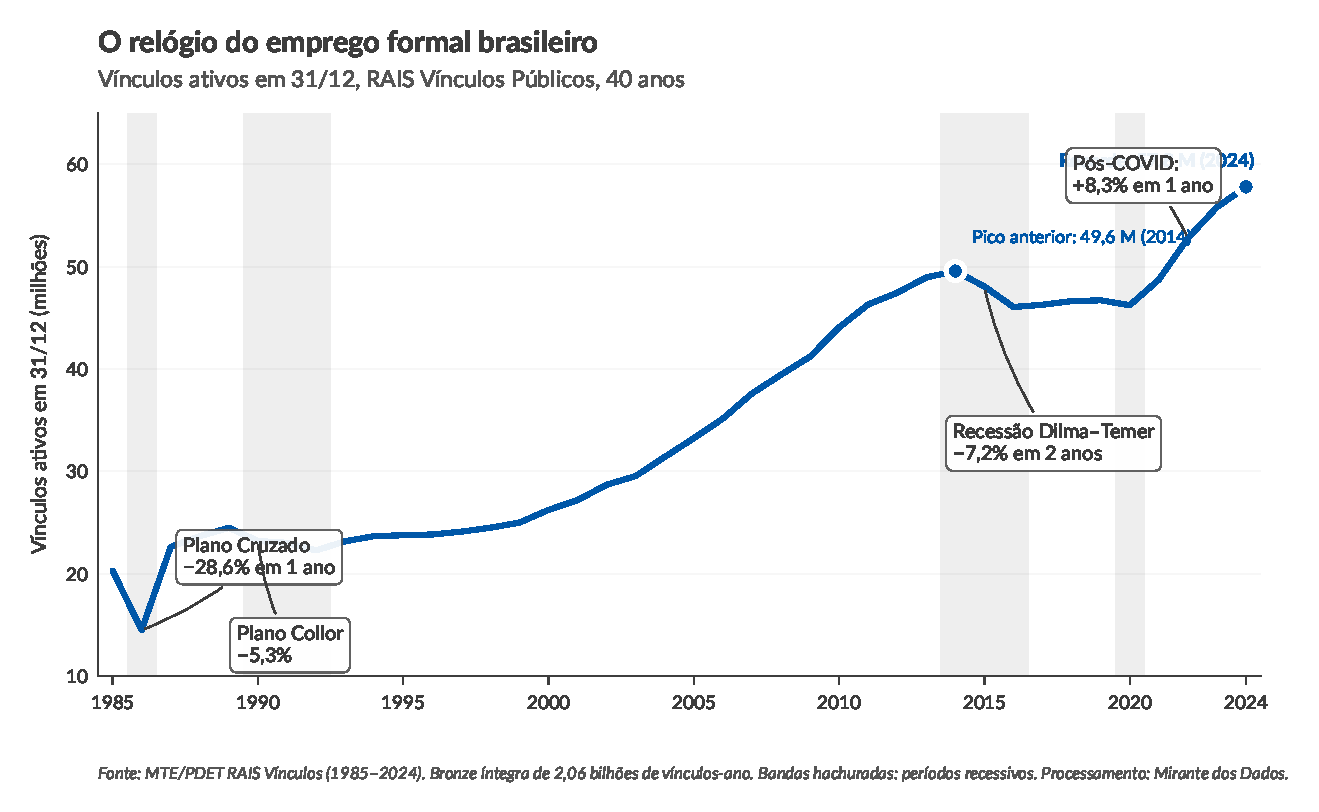
\includegraphics[width=\linewidth]{viz1_relogio_emprego_formal.pdf}
  \caption{O relógio do emprego formal brasileiro, 1985--2024.
  Vínculos ativos em 31/12. Bandas verticais hachuradas indicam
  períodos recessivos. O choque COVID-19 de 2020 ($-1{,}0\%$) é
  notavelmente menor em magnitude que os 3 choques anteriores ---
  evidência preliminar consistente com a hipótese de que o BEm
  preservou empregos formais durante a pandemia.
  \textbf{Fonte:} MTE/PDET RAIS Vínculos (1985--2024), processamento
  Mirante dos Dados.}
  \label{fig:relogio}
\end{figure}

\subsection{Heterogeneidade setorial de exposição ao BEm}

[A inserir após silver populada: tabela de
\texttt{setor\_bem\_exposicao} $\times$ ano com vínculos ativos
e variação percentual. Mostrar que setores ``alta exposição''
caíram mais em 2020 e recuperaram mais em 2021--2022.]

\subsection{Heterogeneidade demográfica}

[A inserir: distribuição de mulheres, baixa escolaridade,
faixas salariais por categoria de exposição BEm.]

% =====================================================================
\section{Resultados}

[Stub. Pendente: rodar modelos sobre silver populada.]

\subsection{Especificação principal}

[Tabela de resultados DiD --- 4 colunas (vínculos ativos, demissões SJC,
massa salarial, demissões pedido) $\times$ 3 painéis (todos os setores,
exposição alta vs baixa, com controles demográficos).]

\subsection{Heterogeneidade}

[Triple-DiD com sexo, escolaridade, porte municipal.]

\subsection{Robustness}

[Placebo, falsification, sensitivity, synthetic control.]

% =====================================================================
\section{Discussão}

[Stub.]

\subsection{Interpretação econômica do efeito estimado}

[Magnitude relativa a outras políticas internacionais; mecanismos
microeconômicos plausíveis.]

\subsection{Custo fiscal vs benefício social}

[Comparação do custo BEm reportado (R\$ 33 bi segundo MTE) com
estimativa de empregos preservados $\times$ valor presente do
seguro-desemprego evitado.]

\subsection{Lições para futuras crises}

[Generalização para outros choques transitórios; pré-anúncio do
desenho de um BEm permanente standby.]

% =====================================================================
\section{Conclusão}

[Stub.]

% =====================================================================
\section*{Reprodutibilidade}

\textbf{Pipeline completo} reproduzível em
\url{https://github.com/leonardochalhoub/mirante-dos-dados-br}.
Bronze, silver e gold do RAIS são tabelas Delta com Apache Iceberg
exposto via Unity Catalog REST endpoint. Análise descritiva
(Seção~\ref{sec:descritivas}) é replicada por commit hash
\texttt{<TBD>} executando \texttt{databricks bundle run job\_rais\_refresh}.

\textbf{Snapshot Delta} usado neste paper:
\texttt{mirante\_prd.bronze.rais\_vinculos@v6} (\textit{Time Travel}
Delta) e \texttt{mirante\_prd.silver.rais\_bem\_panel@v1}.

\textbf{DOI Zenodo:} <a obter no commit final>.

\textbf{ADRs relacionadas:}
\begin{itemize}
  \item ADR-001 --- Bronze RAIS: leitor dual-format per-year
  \item ADR-002 --- Silver TEMÁTICA por questão de pesquisa
  \item ADR-003 --- Grain VINC-only $\cdot$ ausência de CPF na bronze
  \item ADR-004 --- CBO 1994 $\neq$ CBO 2002 $\cdot$ incompatibilidade cross-era
  \item ADR-005 --- Grau de Instrução $\cdot$ drift de codebook 1985$\to$2005$\to$2023
\end{itemize}

% =====================================================================
\section*{Referências}

[A completar após revisão sistemática.]

\end{document}
